\documentclass[a4paper]{article}
\usepackage[utf8]{inputenc}
\usepackage[spanish, es-tabla, es-noshorthands]{babel}
\usepackage[table,xcdraw]{xcolor}
\usepackage[a4paper, footnotesep = 1cm, width=20cm, top=2.5cm, height=25cm, textwidth=18cm, textheight=25cm]{geometry}
%\geometry{showframe}

\usepackage{tikz}
\usepackage{amsmath}
\usepackage{amsfonts}
\usepackage{amssymb}
\usepackage{float}
\usepackage{graphicx}
\usepackage{caption}
\usepackage{subcaption}
\usepackage{multicol}
\usepackage{multirow}
\setlength{\doublerulesep}{\arrayrulewidth}
\usepackage{booktabs}

\usepackage{hyperref}
\hypersetup{
    colorlinks=true,
    linkcolor=blue,
    filecolor=magenta,      
    urlcolor=blue,
    citecolor=blue,    
}

\newcommand{\quotes}[1]{``#1''}
\usepackage{array}
\newcolumntype{C}[1]{>{\centering\let\newline\\\arraybackslash\hspace{0pt}}m{#1}}
\usepackage[american]{circuitikz}
\usetikzlibrary{calc}
\usepackage{fancyhdr}
\usepackage{units} 
\usepackage{svg}

\graphicspath{{../Ejercicio-1/}{../Ejercicio-2/}{../Ejercicio-3/}{../Ejercicio-4/}{../Ejercicio-5/}}
%\svgpath{{../Ejercicio-1/}{../Ejercicio-2/}{../Ejercicio-3/}{../Ejercicio-4/}{../Ejercicio-5/}}

\pagestyle{fancy}
\fancyhf{}
\lhead{22.05 ASSD}
\rhead{Mechoulam, Lambertucci, Rodriguez, Londero}
\rfoot{Página \thepage}

\begin{document}

Se quiere construir el diagrama de tiempos del MC68HC11 para el programa de la Tabla (\ref{prog}).

\begin{table}[H]
\centering
\begin{tabular}{|cccc|}
\hline
 & org & $\$C000$ &  \\
 & ldaa &  & $\#\$A5$ \\
L1 & staa &  & $\$4000$ \\
 & jmp &  & L1 \\
 \hline
\end{tabular}
\caption{Programa a implementar.}
\label{prog}
\end{table}

Para esto, se construye la Tabla (\ref{prog1}) donde se descompone a cada instrucción en los ciclos que la componen.

\begin{table}[H]
\centering
\begin{tabular}{|cccc|}
\hline
Instruction & Cycle & Address & Data \\
LDAA & $1$ & $\$C000$ & $\$86$ \\
$$ & $2$ & $\$C001$ & $\$A5$ \\
STAA & $3$ & $\$C002$ & $\$B7$ \\
$$ & $4$ & $\$C003$ & $\$40$ \\
$$ & $5$ & $\$C004$ & $\$00$ \\
$$ & $6$ & $\$4000$ & $\$A5$ \\
JMP & $7$ & $\$C005$ & $\$7E$ \\
$$ & $8$ & $\$C006$ & $\$C0$ \\
$$ & $9$ & $\$C007$ & $\$02$ \\
\hline
\end{tabular}
\caption{Descomposición en ciclos del programa a implementar.}
\label{prog1}
\end{table}

Finalmente, se construye el diagrama de tiempos teniendo en cuenta el modo extendido del MC68HC11 en el cual el bus de address está compuesto por el puerto C para los ocho bits menos significativos y el puerto B para los ocho bits más significativos. A su vez, el puerto C está multiplexado de manera tal que funcione como bus de datos en el semiciclo bajo de la señal de enable. 

\begin{figure}[H]
  \centering
  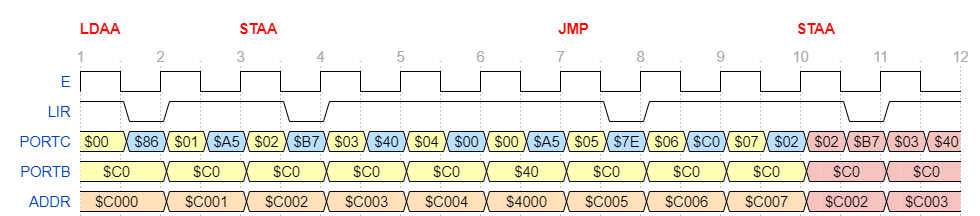
\includegraphics[width=\textwidth]{ImagenesEjercicio5/diagtiempos_5.png}
  \caption{Diagrama de tiempos del programa de la Tabla \ref{prog}.}
  \label{diagtiempos_5}
\end{figure}

La señal de ADDR indica el valor del bus de address visto como la concatenación del puerto C latcheado y el puerto B. La señal de LIR es una señal activa baja de ayuda al momento de debuggear y marca el primer semiciclo negativo de cada ciclo de cada nueva instrucción. Esto es útil debido a que, como se puede ver en la Figura (\ref{diagtiempos_5}), la señal LIR tendrá un valor bajo cuando el puerto C retiene el OPCODE, el cual identifica qué instrucción ejecutará el M68HC11.

\end{document}